\documentclass[letterpaper, 12pt]{article}

 
\usepackage[utf8]{inputenc}
\usepackage[T1]{fontenc} 
\usepackage[french]{babel}
\usepackage{amsmath}
\usepackage{textcomp}
\usepackage{tocloft}

\usepackage[letterpaper, left=2.5cm, right=2.5cm, top=2.5cm, bottom=2.5cm]{geometry}
\usepackage{graphicx}
\usepackage{float} 
\usepackage{setspace} 
\usepackage{fancyhdr}      
\usepackage{cite}

\usepackage[pdftex, colorlinks=true, linkcolor=black, citecolor=blue]{hyperref}

\title{Proposé de recherche}
\author{Thomas Dändliker}
\date{\today}

\pagestyle{fancy}
\fancyhead[L]{Proposé de recherche}
\fancyhead[R]{MET-7900}

%%%%%%%%%%%% Fin du préambule %%%%%%%%%%%

\begin{document}

\begin{titlepage}
	\newcommand{\HRule}{\rule{\linewidth}{0.2mm}}     
	
	\begin{figure}[t]
		\begin{minipage}{0.5\textwidth}\large
			\begin{flushleft}
				
\includegraphics[width=5cm]{ULAVAL}
			\end{flushleft}
		\end{minipage}
		\begin{minipage}{0.5\textwidth}\large
			\begin{flushright}
				
\includegraphics[width=6cm]{CRMR}
				
			\end{flushright}
		\end{minipage}
	\end{figure}
	\textsc{ \\[1cm]}
	
	% Titre
	\begin{center}
		\HRule 
		\\[0.5cm]
		{\Large    \textbf{Optimisation de la densité de reboisement en fonction des grades de qualité des bois sciés}}
		\HRule
		\\[0.5cm]
		{\large Proposé de recherche \\
		}
		
	\end{center}
	
	\vfill 
	\begin{center}
		
		\textsc{\large      
			Université Laval\\
			Faculté de foresterie, de géographie et de géomatique\\[3cm]}
	\end{center}

	
	\begin{minipage}{0.5\textwidth}
		\begin{flushleft} \large
			\emph{Auteur:}\\
			Thomas Dandliker 
		\end{flushleft}
	\end{minipage}
	~
	\begin{minipage}{0.5\textwidth}
		\begin{flushright}\large
			\emph{Superviseurs:} \\
			Alexis Achim \\
			Charles Ward \\
		\end{flushright}
	\end{minipage}
	
\end{titlepage}


\renewcommand{\contentsname}{\hfill\bfseries\LARGE Table des matières\hfill} 
\renewcommand{\listfigurename}{\hfill\bfseries\LARGE Table des figures\hfill} 

%%%%%%%%% Table des matières %%%%%%%%%%%

\newpage
\doublespacing
\setcounter{tocdepth}{3}
\tableofcontents
\addtocontents{toc}{\vspace{2cm}}

%%%%%%%%% Table des figures %%%%%%%%%%

\newpage
\doublespacing
\listoffigures

\newpage
\section{Introduction}
\begin{onehalfspace}

Les forêts issues de plantation comptent pour 4\% des forêts mondiales, mais fournissent, à elles seules, 50\% de la production de bois \cite{Miller2009}. Précisons qu'au Québec, pour la période de 2001 à 2012, avec environ 120 millions de plants plantés annuellement, les résineux représentent presque la totalité des plantations de la province, soit 98\% \cite{Richard2015}. Depuis 2001, 94\% des plantations y sont réalisées avec trois essences: l'épinette noire 56\% (\textit{Picea mariana} (Mill.)), le pin gris 21\% (\textit{Pinus banksiana} (Lamb.)) et l'épinette blanche 17\% (\textit{Picea glauca}), comme l'illustre la figure \ref{proportion}:

\vspace{12pt}

\begin{figure}[h]
	\centering
	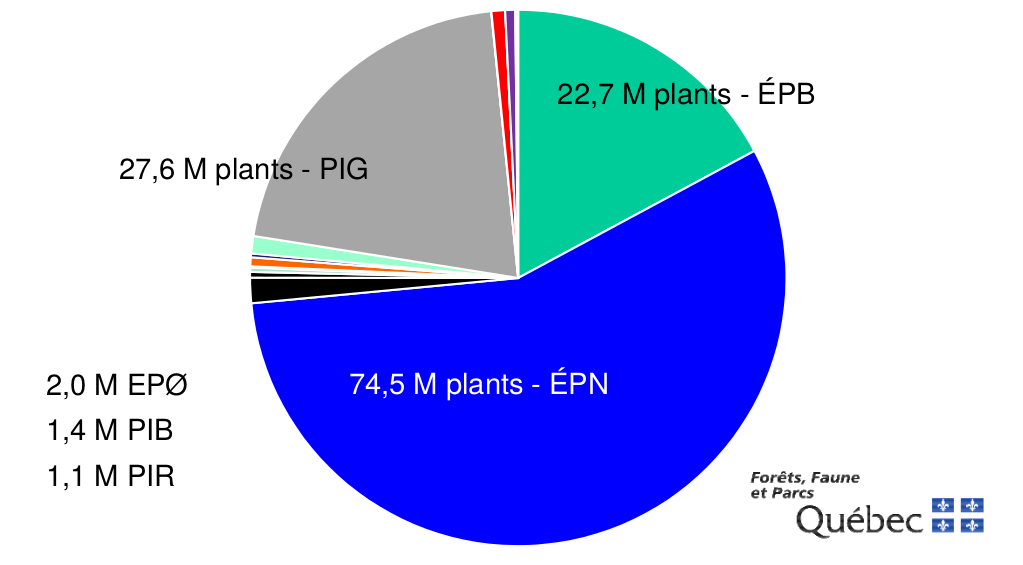
\includegraphics[width=12cm]{Essencesplantees}
	\caption{Essences plantées entre 2001 et 2012 au Québec}
	\label{proportion}
\end{figure}


Ces trois essences font partie du groupe dit SEPM (Sapin, Épinettes, Pins, Mélèzes), qui constitue la  majeure  partie  des  volumes  de  bois  récoltés et transformés au Québec. Ce groupe est à la base de l’approvisionnement des usines produisant du sciage\cite{Gouv2017}. Dans un marché globalisé, cela implique d'optimiser les procédés qui englobent toutes la chaîne de valeur du bois, y compris les scénarios sylvicoles \cite{Gaudreault2010}. 

\subsection{Forte densité \textit{versus} faible densité de plantation}

Dans ce cadre de rationnalisation, la densité de plantation est un outil de grande influence en sylviculture, puisqu'elle détermine la croissance et les caractéristiques du peuplement \cite{Thiffault2003}. Il est à noter que la hauteur dominante - une de ces caractéristiques - n'est généralement pas influencée par l'espacement entre les tiges \cite{Gizachew2012}. En revanche, lorsque le nombre de tiges par hectare augmente, on a pu observer des augmentations du volume total et de la surface terrière, et, dans le même temps, une diminution du diamètre quadratique moyen. Il est ainsi reconnu que le DHP d'un arbre est étroitement lié à la densité de plantation \cite{Pregent1998}. De plus, en densité élevée, la mortalité y est aussi plus forte, due à une compétition intraspécifique plus élevée \cite{Groot2016, Will2010}. À l'inverse, à plus faible densité de plantation, on constate un meilleur taux de survie, ainsi qu'une plus forte croissance en diamètre et en volume par tige \cite{Akers2013}. À cela, on constate une gradation du taux de survie en fonction de l'indice de qualité de station (IQS)  pour l'épinette blanche \cite{Pregent2010}. Plus la la fertilité augmente la mortalité s'accentue.

\vspace{12pt}

\begin{figure}[h]
	\centering
	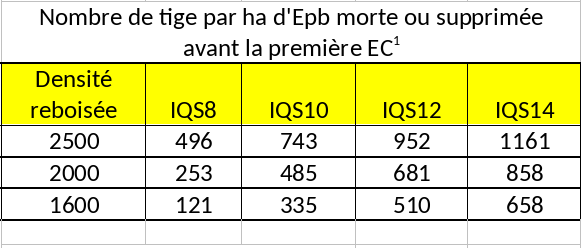
\includegraphics[width=12cm]{IQS}
	\caption{Nombre de tige par ha d'Epb mortes ou supprimées avant la première éclaircie \cite{Pregent2010}}
	\label{iqs}
\end{figure}

\vspace{12pt}

À faible densité de plantation, on observe également une augmentation du défilement (conicité). Ce dernier aspect a une incidence directe sur le volume marchand des tiges. En effet, pour un même diamètre donné, un fort défilement diminue le volume marchand à l'échelle de l'arbre\cite{Pregent1998}. Mais en parallèle, un des avantages de cette faible densité est une croissance radiale plus rapide ; ce qui permet de transformer une plus forte proportion du volume en planche \cite{Auty2014}. D'où la nécessité de rechercher un \textit{optimum}, entre un défilement acceptable et un bon accroissement diamétral.

\vspace{12pt}

Ainsi, trois facteurs entrent en compte lors de la première transformation d'un arbre: le diamètre, la hauteur totale et le défilement. Ces trois caractéristiques influent sur la composition du panier de produits sciés \cite{Auty2014}, comme par exemple la proportion de sciage.

\subsection{Panier de produits}

Dans un contexte de marché de plus en plus compétitif, et où les coûts d'extraction pour la ressource et la fabrication des produits du bois augmentent, il devient primordial de maximiser la création de valeur lors de la première transformation \cite{Briggs2010, Walker2013}. Cela est particulièrement pertinent dans la forêt boréale de l'est du Canada, puisque le petit diamètre des tiges récoltées limite les dimensions du bois d'œuvre. Depuis plusieurs décénnies, des simulateurs informatiques de sciages sont utilisés dans le secteur des transformations primaire et secondaire comme stratégie d'optimisation de la valeur des produits \cite{FPInnovations2014}. Certaines études ont intégré avec succès les variabilités de la taille des arbres (tels que le diamètre de la tige, la hauteur totale de l’arbre ou la conicité de la tige) dans des modèles permettant de prédire le volume ou la valeur lors du processus de transformation \cite{Barrette2012,Liu2007}.

\vspace{12pt}

Par ailleurs, l'accroissement plus élevé que l'on constate en plantation modifie les caractéristiques du bois et, de ce fait, a un effet déterminant quant à la valeur et à l'utilisation finale du produit \cite{Zhang2002}. Une manière d'attribuer une valeur pour les résineux consiste à effectuer un classement visuel des bois sciés comme le fait la norme "National Lumber Grades Authority (NLGA)". Elle indique que les nœuds (branches), précisément leurs tailles et leurs nombres, sont des caractéristiques importantes à prendre en considération lors du classement des bois sciés \cite{Lemieux2000}.

\subsection{Branchaison \textit{versus} qualité des bois sciés}

L'espacement initial a un effet déterminant sur les coûts d'établissement de la régénération, sur la croissance des arbres et sur le rendement du peuplement. En détail, la densité de plantation affecte la structure de la couronne, la taille de la branche ainsi que les caractéristiques du bois produit. Par conséquent, les décisions relatives à l'espacement initial impacteront non seulement la valeur du peuplement et le retour sur investissement, mais aussi la qualité des produits issus de la plantation.

\vspace{12pt}

Sachant que la première partie de la bille est la plus rémunératrice, c'est aussi elle qui contient certains défauts de déclassement de la qualité des bois sciés, notamment, les branches grosses et mortes. Pour le pin gris et l'épinette blanche, l'espacement des plantations a un effet significatif sur le diamètre de la plus grosse branche de l'arbre, et a en outre tendance à augmenter la grosseur des noeuds \cite{Hebert2016, Tong2013}. Dans l'ordre, la densité de plantation influe le DHP ; le DHP influe ensuite sur les caractéristiques des branches. En suivant ce raisonnement, le sylviculteur peut agir sur la branchaison en remontant à l'origine, c'est-à-dire en choisissant la densité de plantation.

\vspace{12pt}

Ainsi, les attributs des nœuds peuvent être prédits pour le pin gris et l’épinette noire à partir d'observations visuelles des branches, notamment leurs grosseurs \cite{Duchateau2013}. De plus, pour un site donné, les propriétés des noeuds d'épinette noire  sont relativement peu sensibles à l'espacement des arbres, car elles sont largement expliquées par la taille du fût ainsi que celle du houppier \cite{Benjamin2009, Zhang2005}. Cela est également observé sur l'épinette de Norvège en Scandinavie \cite{Johansson1992, Makinen1999, Pfister2007}. Enfin, le diamètre de la plus grande branche est positivement corrélé au DHP de l'arbre, quel que soit l'espacement entre les arbres \cite{Hebert2016, Tong2005}. 

\vspace{12pt}
 
Donc, aux vues de ces connaissances, le sylviculteur a une réelle emprise sur la qualité du bois dès sa première décision, qui est celle de choisir la densité de plantation. D'une part, un espacement initial élevé aura l'avantage de stimuler la croissance diamétrale des tiges, ce qui favorisera la production de bois de sciage sur de plus courtes révolutions. D'autre part, le défilement plus élevé et la taille plus élevées des nœuds qui découlent de tels espacements initiaux est susceptible de diminuer le rendement en sciage, leur grade de qualité, et donc la valeur des bois produits. Les sylviculteurs québécois n'ont présentement pas d'outils à leur disposition leur permettant d'évaluer où se situe l'\textit{optimum} d'espacement initial qui maximiserait la valeur des bois produits.

\subsection{Objectifs de l'étude}

Les études menées préalablement sur les branches sont, pour l'instant, toutes limitées à un site en particulier avec des conditions de croissance bien définies (indice de qualité de station, précipitation, température, etc.). De surcroît, les études évaluant la proportion de sciage proviennent de jeunes peuplements résineux qui ne sont pas encore arrivés à maturité, donc n’ayant pas suivi un scénario sylvicole complet - ­avec ou sans éclaircies. Pour pallier le manque d'un portrait plus général, la présente étude s’appuie sur un réseau de placettes permanentes établies dans des plantations s'approchant de la maturité à l’échelle de la province du Québec, ce qui permettra de couvrir de nombreux types de stations ayant des conditions de croissance différentes. 

\vspace{12pt}

Le présent projet vise à établir un lien entre la future qualité du bois scié et la croissance des arbres à différents espacements pour trois espèces commerciales du Canada, soit l'épinette noire, l'épinette blanche et le pin gris. L'objectif précis de l'étude est alors d'évaluer l'effet de différents espacements sur les propriétés du bois d'arbres arrivés à maturité. Plus particulièrement, nous avons cherché à déterminer si une réponse positive du DHP à un espacement plus grand affecterait le classement du bois et la proportion de sciage.

\subsection{Hypothèse}

Nous avons émis l'hypothèse qu'une densité de reboisement plus faible que celui appliqué présentement au Québec, soit 2 m, augmenterait le diamètre à l'échelle de l'arbre, ce qui augmenterait le rendement en sciage sans diminuer outre mesure le classement des sciages. Cette hypothèse implique donc que l'\textit{optimum} de rendement en valeur des produits se situerait à un espacement initial inférieur à celui utilisé en ce moment. 

\section{Matériels et méthodes}

\subsection{Aire d'étude}

L'expérience sera réalisée à l'échelle de la province du Québec et elle mettra à profit le réseau des placettes permanentes de la Direction de la Recherche Forestière (DRF). Le Service de la sylviculture et du rendement des forêts (SSRF) dispose en effet d'un programme de suivi des plantations s'intitulant "Effets réels des traitements sylvicoles en plantations". Ce programme qui vise à modéliser la croissance et le rendement des plantations s'appuie sur plus de 500 placettes. Tous les cinq ans, on y mesure différentes caractéristiques du peuplement et des arbres. Dans le cadre de cette étude, les essences étudiées sont l'épinette noire, l'épinette blanche et le pin gris. Des mesures préliminaires ont été prises durant l'été et l'automne 2018 ; elles seront complétées au printemps et à l'été 2019 dans une centaine de plantations monospécifiques. L'ensemble des plantations ont été établies en 1986  avec  des  plants  produits  à  racines  nues  et  à  des  densités  de  reboisement  variant  de  1111  à  4444  plants  à  l’hectare. Tous les arbres sont  âgées  de  32 ans  au  moment  de  la  prise  de  mesures. De plus, toutes les plantations sélectionnées n'ont subi aucune éclaircie précommerciale. Au total, 174 placettes seront mesurées parmi le réseau des placettes permanentes (Figure \ref{local}). La sélection des placettes demeure à préciser.  % J'attends une réponse de Charles pour connaître la méthode de sélection des placettes année après année

\vspace{12pt}

\begin{figure}[H]
	\centering
	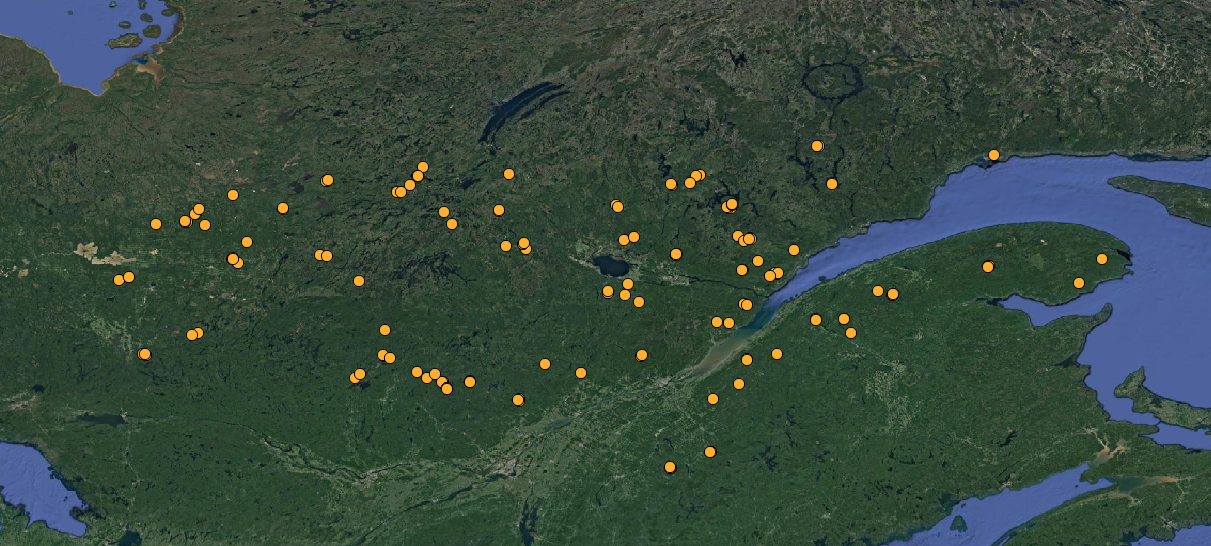
\includegraphics[width=13cm]{Localisation}
	\caption{Localisation des plantations à mesurer pour 2018-2019}
	\label{local}
\end{figure}

Les placettes permanentes utilisées sont des unités d'échantillonnage circulaires d'une superficie de 400 m$^{2}$ \cite{MFFP2016}. À son cinquième cycle de mesurage en 2018, le protocole d'inventaire existant a été modifié pour inclure des mesures de branches. Les données suivantes seront relevées sur les arbres: l'essence de l'arbre, le diamètre à hauteur de poitrine (DHP) et les caractéristiques de la plus grosse branche sur les cinq premiers mètres de la tige. 

\subsection{Mesures de branches}

\subsubsection{Critères de sélection des tiges}

L'objectif premier est de pouvoir sélectionner des tiges qui sont prédisposées à perdurer dans le peuplment jusqu'à la fin d'un scénario sylvicole. Pour rappel, les plantations sélectionnées dans cette étude n'ont pas encore été traitées. Pour prendre en compte les futurs éclaircies à venir dans la sélection des tiges, une éclaircie "fictive" est simulée. Les critères de sélection de cette intervention sont essentiellement le DHP, la présence de maladies et de défauts. 

\vspace{12pt}

Au niveau dendrométrique, il a été convenu que les tiges actuelles doivent avoir un DHP supérieur au DHP moyen. Ce critère permet de soustraire les tiges opprimées et intermédiaires qui n'ont pas de chance de se développper à leurs plein potentiel à moyen et long terme. 

\vspace{12pt}

L'aspect sanitaire est également imporant à prendre en considération car il peut, d'une part compromettre la survie de la tige, et d'autre part impacter négativement la croissance et la qualité interne de la bille. Les maladies et les insectes suivants ont été considérées comme préjudiciables pour la sélection des tiges:

\vspace{12pt}

\begin{itemize}

\item Rouille vésiculeuse du Pin gris;
\item Chancre;
\item Chancre hypoxylonien;
\item Chancre avec pourriture;
\item Champignons et consoles;
\item Carpophore;
\item Nodulier;
\item Perceur d'écorce;
\item Becquetage d'oiseaux.
	
\end{itemize}

\vspace{12pt}

Le dernier critère cherche à exclure les défauts visuels qui sont susceptibles de déclasser la première bille de pied, c'est-à-dire le premier 16 pieds (figure \ref{defaut}).  

\vspace{12pt}

\begin{figure}[H]
	\centering
	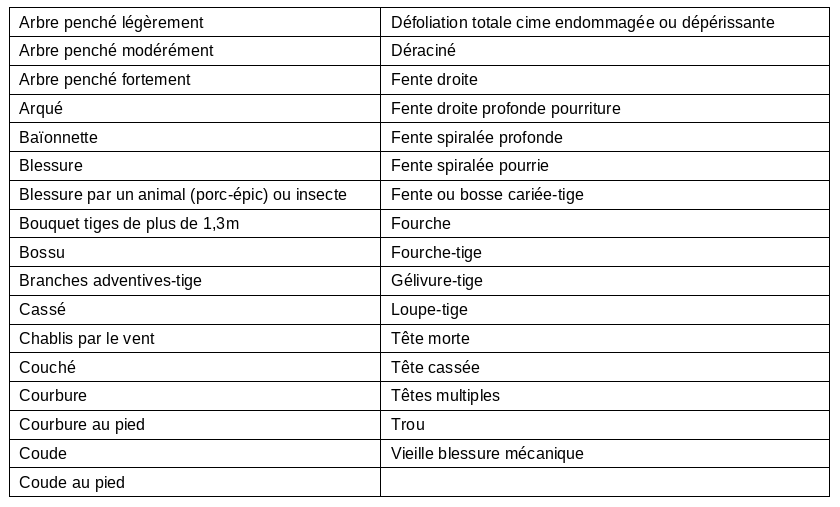
\includegraphics[width=15cm]{Defauts}
	\caption{Liste des défauts visuels impactant le premier 16 pieds}
	\label{defaut}
\end{figure}

\subsubsection{Sélection des tiges dans les placettes}
 
Au total, il est prévu d'inventorier 20 tiges par placette. Ce nombre a été fixé pour faire un compromis, entre, d'une part, le temps de mesurage nécessaire sur le terrain et, d'autre part, la prise en considération de la variabilité des tiges au sein du peuplement. La taille de l'échantillon n'est pas plus élevé, car il s'agit de plantation monospécifique, où l'on s'attend à une plus grande homogénéité des conditions de croissance comparativement à la forêt naturelle. 

\vspace{12pt}

Pour atteindre les critères de sélection et le nombre de tiges à mesurer, l'étude se basera, en premier lieu, sur 10 arbres identifiés préalablement par la DRF. Il s'agit d'arbres études compris dans les étages dominants et codominants (figure \ref{etages}). Ainsi, un arbre est dominant (code D sur la figure \ref{etages}), lorsque sa hauteur dépasse visiblement l'espace occupé par les codominants (code C sur la figure \ref{etages}). Sa  cime s’étend par-dessus l’étage général du couvert principal \cite{Methot2014}. Un codominant est un arbre qui occupe l'espace, où se trouve la majorité des hauteurs d'arbres d'un peuplement, soit approximativement supérieur aux deux tiers de la hauteur des dominants \cite{Methot2014}. Ces 10 arbres sont répartis aléatoirement dans la placette et sont identifiés par un numéro. 

\vspace{12pt}

\begin{figure}[H]
	\centering
	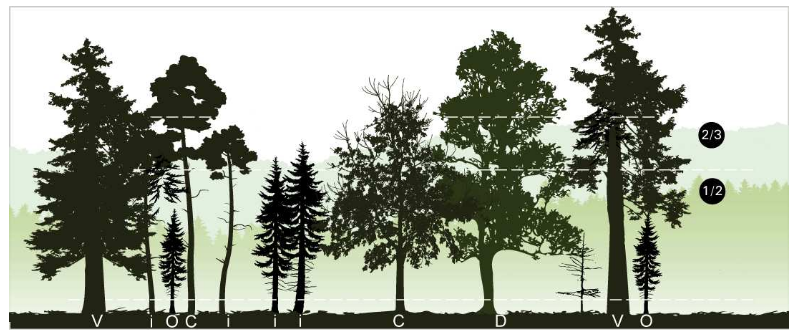
\includegraphics[width=15cm]{etages}
	\caption{Étages d’arbres  vivants sur pied d'essences commerciales}
	\label{etages}
\end{figure}

\vspace{12pt}

Les dix autres arbres proviendront d'une liste respectant les quatre critères de sélection. En prévision du fait que certains défaut auront apparu sur les arbres après le dernier mesurage effectué dans les placette, une liste sera construite de tous les arbres respectant les quatre critères de sélection.
Cette liste servira à compléter la sélection des arbres jusqu’à une concurrence de 20 arbres et elle n’est pas triée en ordre prioritaire de sélection. Les arbres sont sélectionnés prioritairement sur la ligne à proximité du centre de la placette (ligne en rouge et pleine sur la Figure \ref{select}), suivi sur la ligne le plus vers le nord magnétique, suivi sur les lignes adjacentes jusqu’à atteindre la ligne centrale de la placette  (lignes en bleu sur  la Figure \ref{select}) et, si nécessaire, sur les autres lignes adjacentes à la ligne du centre et en priorisant toujours celles orientées vers le nord magnétique (lignes en jaune sur la Figure \ref{select}).

\vspace{12pt}

\begin{figure} [H]
	\centering
	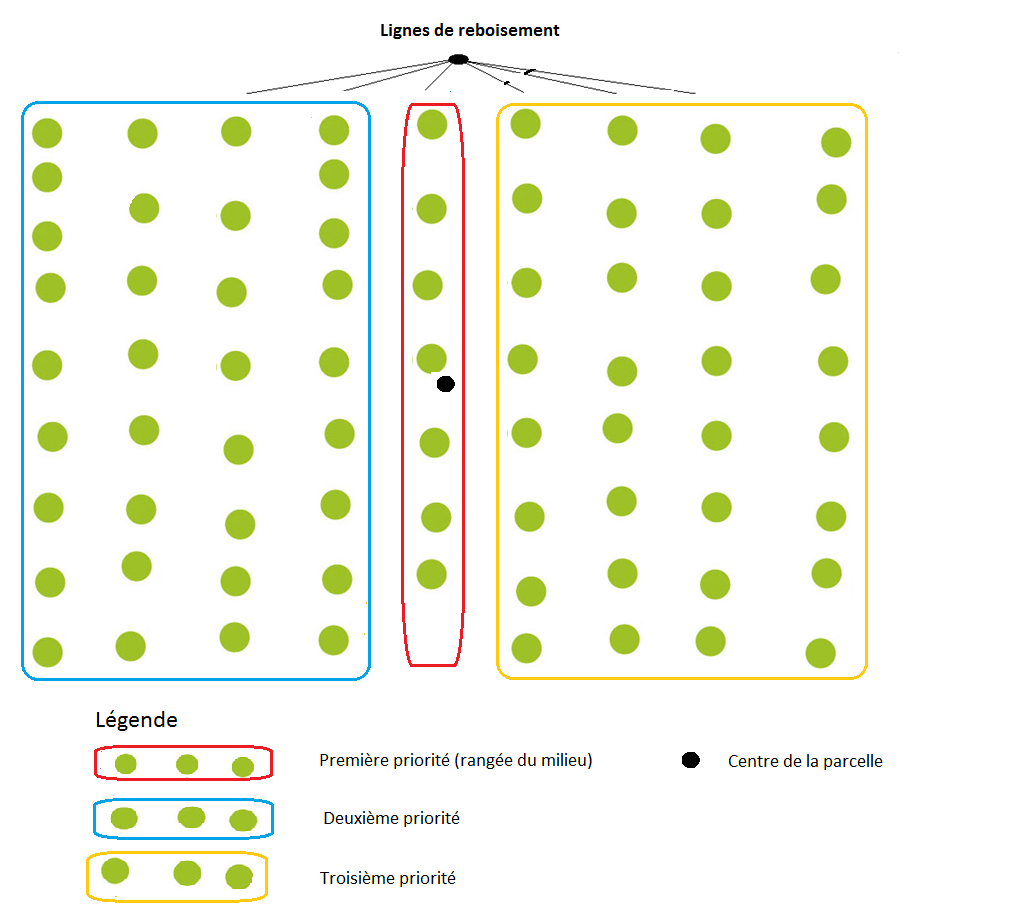
\includegraphics[width=14cm]{Figure1}
	\caption{Priorité de sélection des arbres pour la classification des branches}
	\label{select}
\end{figure}

\vspace{12pt}

\subsubsection{Mesures à l'échelle de l'arbre}

Pour chaque arbre sélectionné, la circonférence de la bille de pied de 4,9 m (16 pieds) sera ensuite divisée en quatre faces égales (Figure \ref{face}). Les faces A et C seront alignées sur la ligne de plantation et les faces B et D seront donc perpendiculaires à la ligne de plantation. La face A sera celle orientée le plus vers le nord magnétique et elle est identifiée par un trait de peinture vertical de 10 cm, à la base du tronc, à l’aide de peinture.

\vspace{12pt}

\begin{figure}[H]
	\centering
	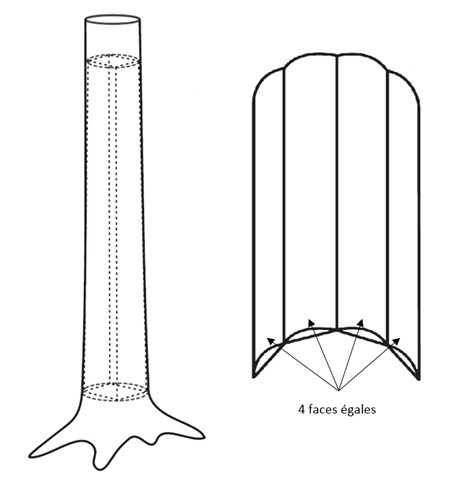
\includegraphics[width=6cm]{Figure2}
	\caption{Division de la circonférence de la bille de pied en quatre faces égales}
	\label{face}
\end{figure}

\vspace{12pt}

Le diamètre de la plus grande branche sera ensuite mesuré sur chacune des faces, selon les six classes suivantes: 

\begin{figure}[H]
	\centering
	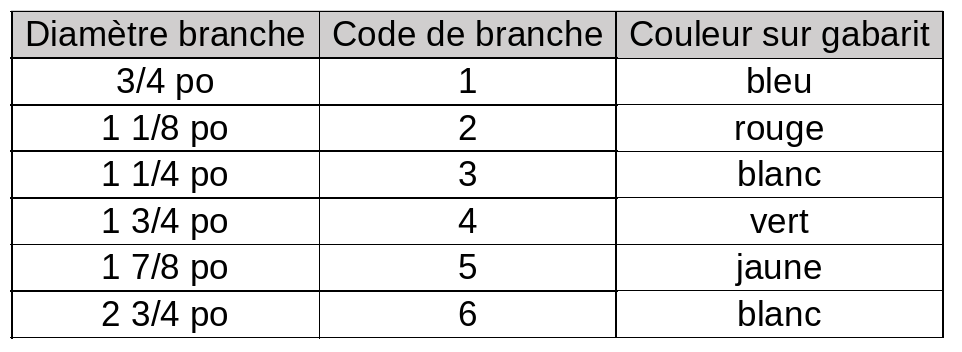
\includegraphics[width=10cm]{Code}
	\caption{Code de branche en fonction du diamètre de la branche}
	\label{code}
\end{figure}

Ces classes de diamètre s’appuient sur les critères de classification NLGA de la qualité des planches. Six dimensions sont retenues, celles associées aux grades sélect, No 2 et No 3 (figure \ref{nlga}). On peut s’abstenir des dimensions du grade No 1 car habituellement le bois est vendu No 2 et meilleur. Nous avons convenu que les orientations de reboisement seront basées sur les deux produits les plus fabriqués pour le marché nord-américain, les 2 x 4 et les 2 x 6. 

\begin{figure}[H]
	\centering
	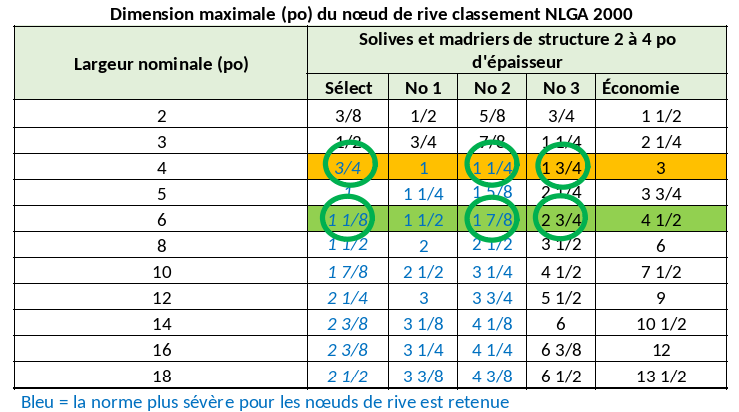
\includegraphics[width=14cm]{NLGA}
	\caption{Dimension maximale (po) du nœud de rive classement NLGA 2000}
	\label{nlga}
\end{figure}

\vspace{12pt}

De plus, deux autres mesures seront prises sur chaque face: l'état de la branche et l'inclinaison de la branche par rapport à la tige. Ces données permetteront d'avoir une caractérisation plus fine de la plus grosse branche mesurée. Si la branche est encore vivante, c'est-à-dire que les aiguilles sur la branche sont vertes ou pas, il sera possible de savoir si elle continuera de grossir dans les années subséquentes ou non. L'inclinaison de la branche quant à elle sera aussi mesurée visuellement. Plus la branche est à insertion aiguë, plus il sera probable qu'elle aura un impact sur le fil du bois et par conséquent, sur les propriétés du bois.

\subsubsection{Protocole}

La plus grosse branche sera sélectionnée jusqu’à une hauteur de 5,23 m (17 pieds), à partir du sol, et par la suite mesurée à l’aide du gabarit métallique. À cet effet, des perches télescopiques et du gabarit métallique (figure \ref{gabarit}), identifiant les six classes de diamètres de branches, ont été fournies aux personnes qui réaliseront les mesures.

\vspace{12pt}

\begin{figure}[H]
	\centering
	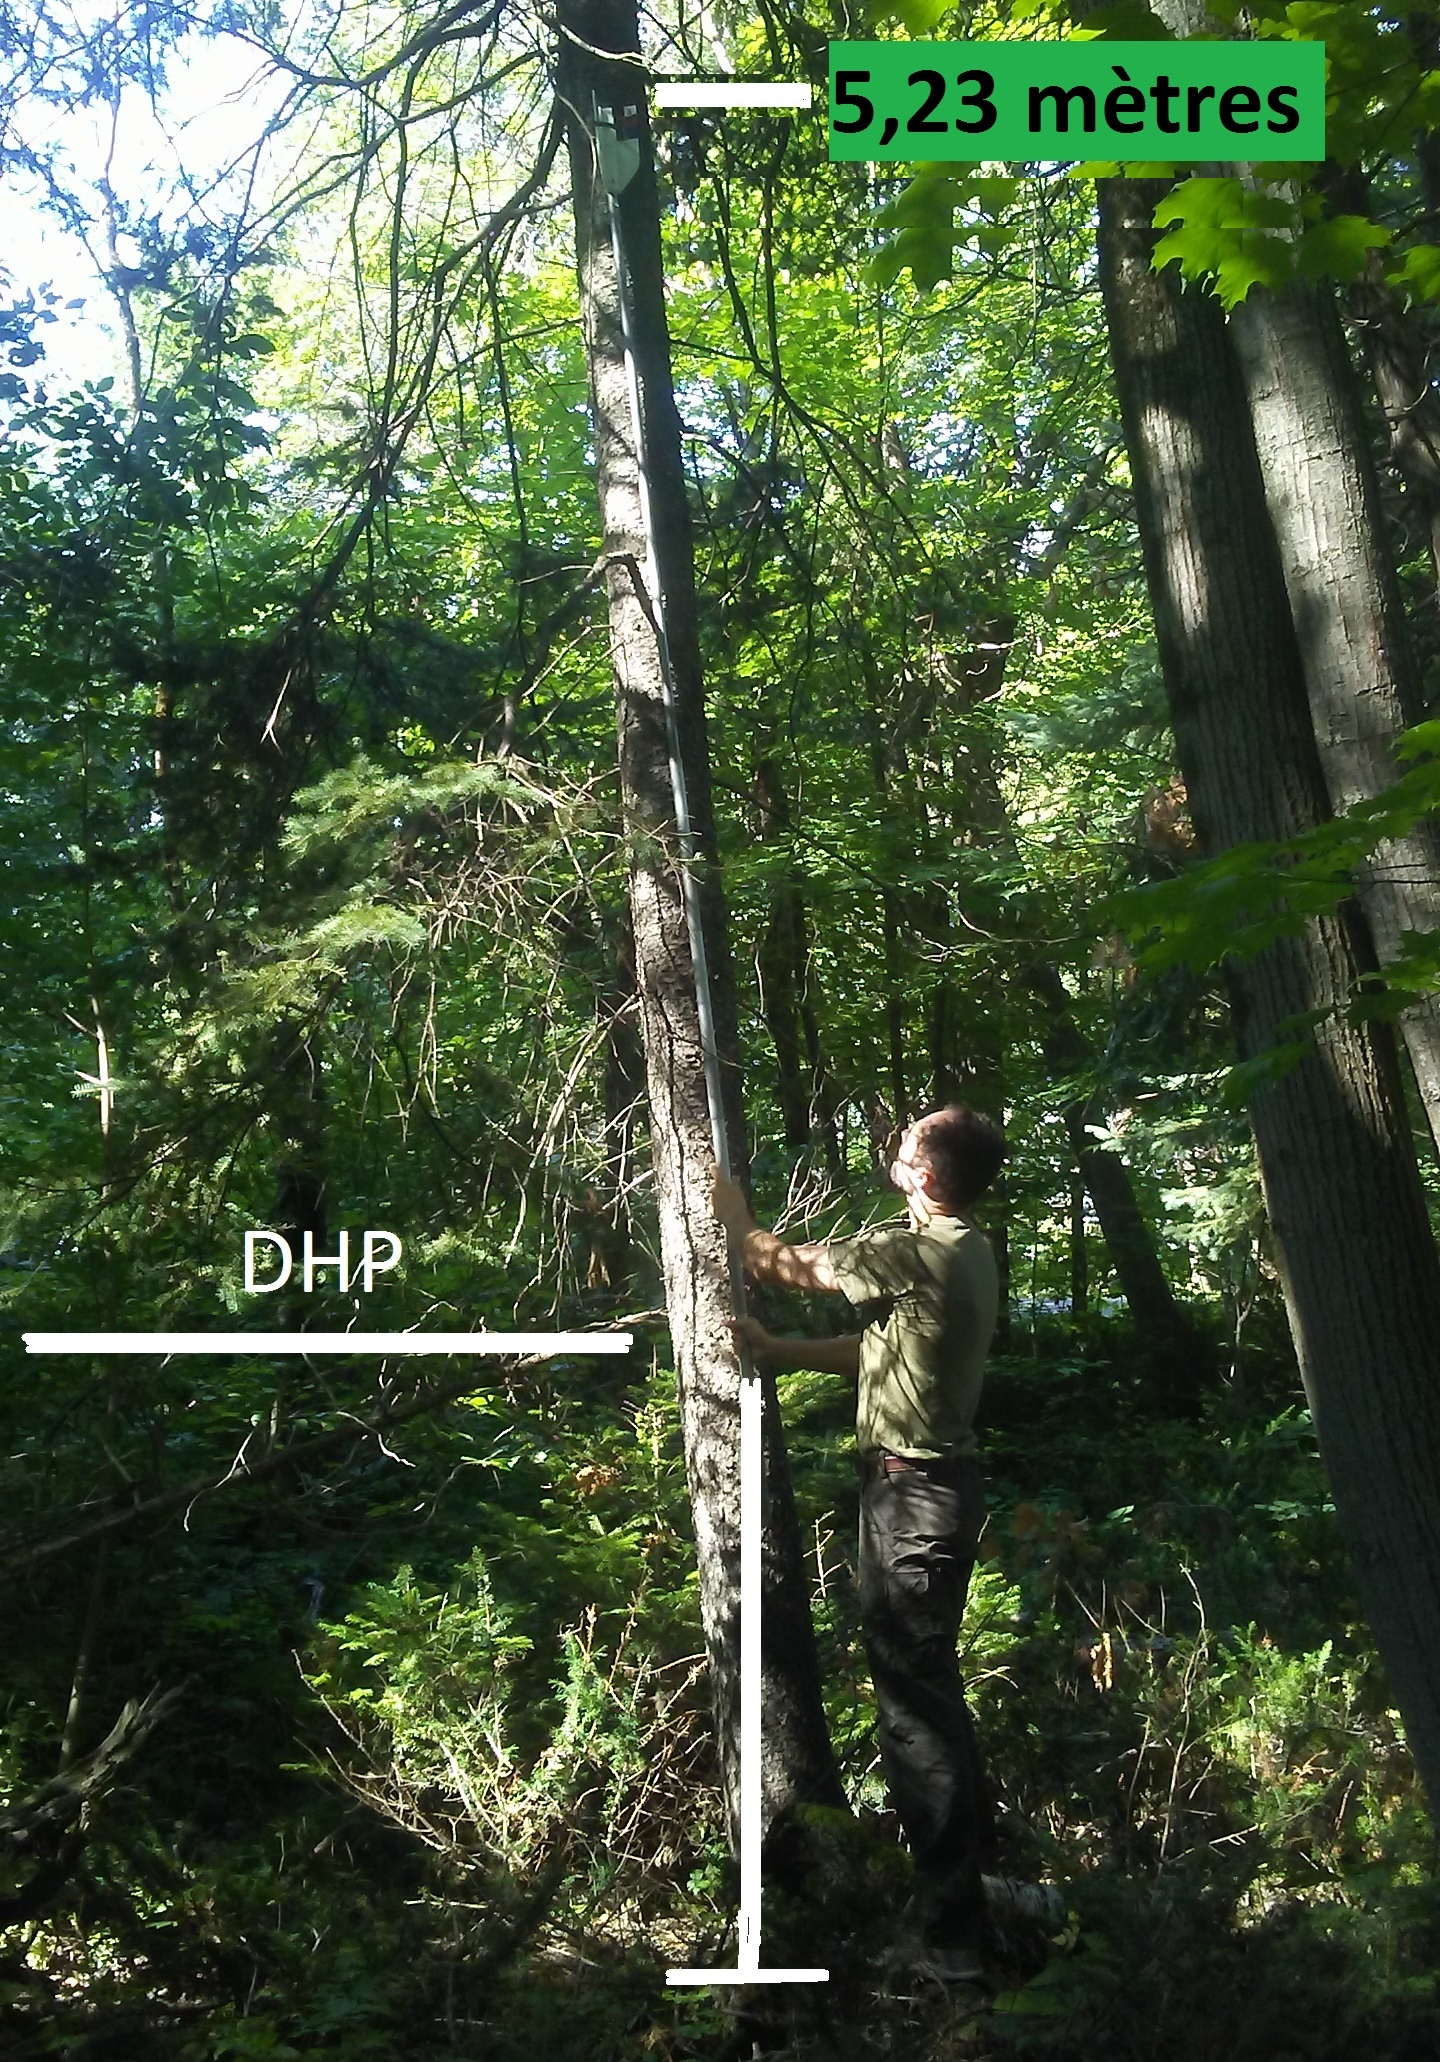
\includegraphics[width=6cm]{Figure5}
	\caption{Détermination de la hauteur de 5,23 m}
	\label{determination}
\end{figure}

\vspace{12pt}

En appliquant ce gabarit à la plus grosse branche de la bille de pied sur chaque face de l’arbre, on peut estimer le grade des planches associé à la grosseur des nœuds. Bien que cet estimé ne donne pas une réponse parfaite, nous avons convenu qu’il est suffisant pour nous guider dans nos choix sylvicoles. Cette méthode est appliquée à l’âge de la première éclaircie commerciale essentiellement à des branches mortes qui ne croitront plus.

\vspace{12pt}

La mesure des branches se décline comme suit:

\begin{enumerate}
	
\item Déployer la perche téléscopique pour atteindre une longueur de 3,93 m. Cette longueur correspond à la longueur totale de la perche sans le gabarit. Ainsi elle débute au niveau du trait rouge présent sur le gabarit métallique (Figure \ref{gabarit}) jusqu'à l'autre extrémité de la perche téléscopique.

\item Se placer devant la face à mesurer avec la perche téléscopique munie du gabarit métallique.

\item Positionner la base de la perche à  1,3 m du sol : prendre la perche téléscopique par la base, et la soulever jusqu'au niveau du DHP, identifié par un trait de peinture sur l'arbre (Figure \ref{determination}). Cette position permet de délimiter la hauteur totale de 5,23 m, hauteur qui sert à étudier les branches.

\item Chercher la branche la plus grosse sur la face étudiée et la mesurer à l’aide du gabarit métallique (Figure \ref{gabarit}). Inscrire dans le formulaire Dendrodif le «code diamètre branche» selon le tableau ci-dessus (figure \ref{code}), correspondant à la plus grosse branche. Pour chacune des branches, identifier et inscrire dans le formulaire Dendrodif, son «état branche» : vivante = \textbf{V}, ou morte = \textbf{M}.  De plus, inscrire dans le formulaire Dendrodif, son «angle insertion branche» : 45° et moins = \textbf{- 45}, ou 45° et plus = \textbf{+ 45}.

\end{enumerate}

\vspace{12pt}
 
Voir exemple ci-dessous de prise de mesures dans le formulaire Dendrodif :

\vspace{12pt}

\begin{figure}[H]
	\centering
	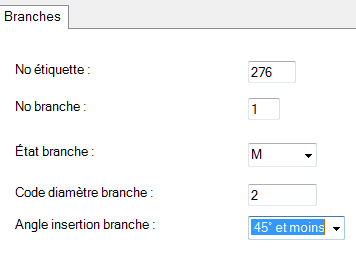
\includegraphics[width=5cm]{Figure3}
	\caption{Interface DendroDif}
\end{figure}

\vspace{12pt}

\begin{figure}[H]
	\centering
	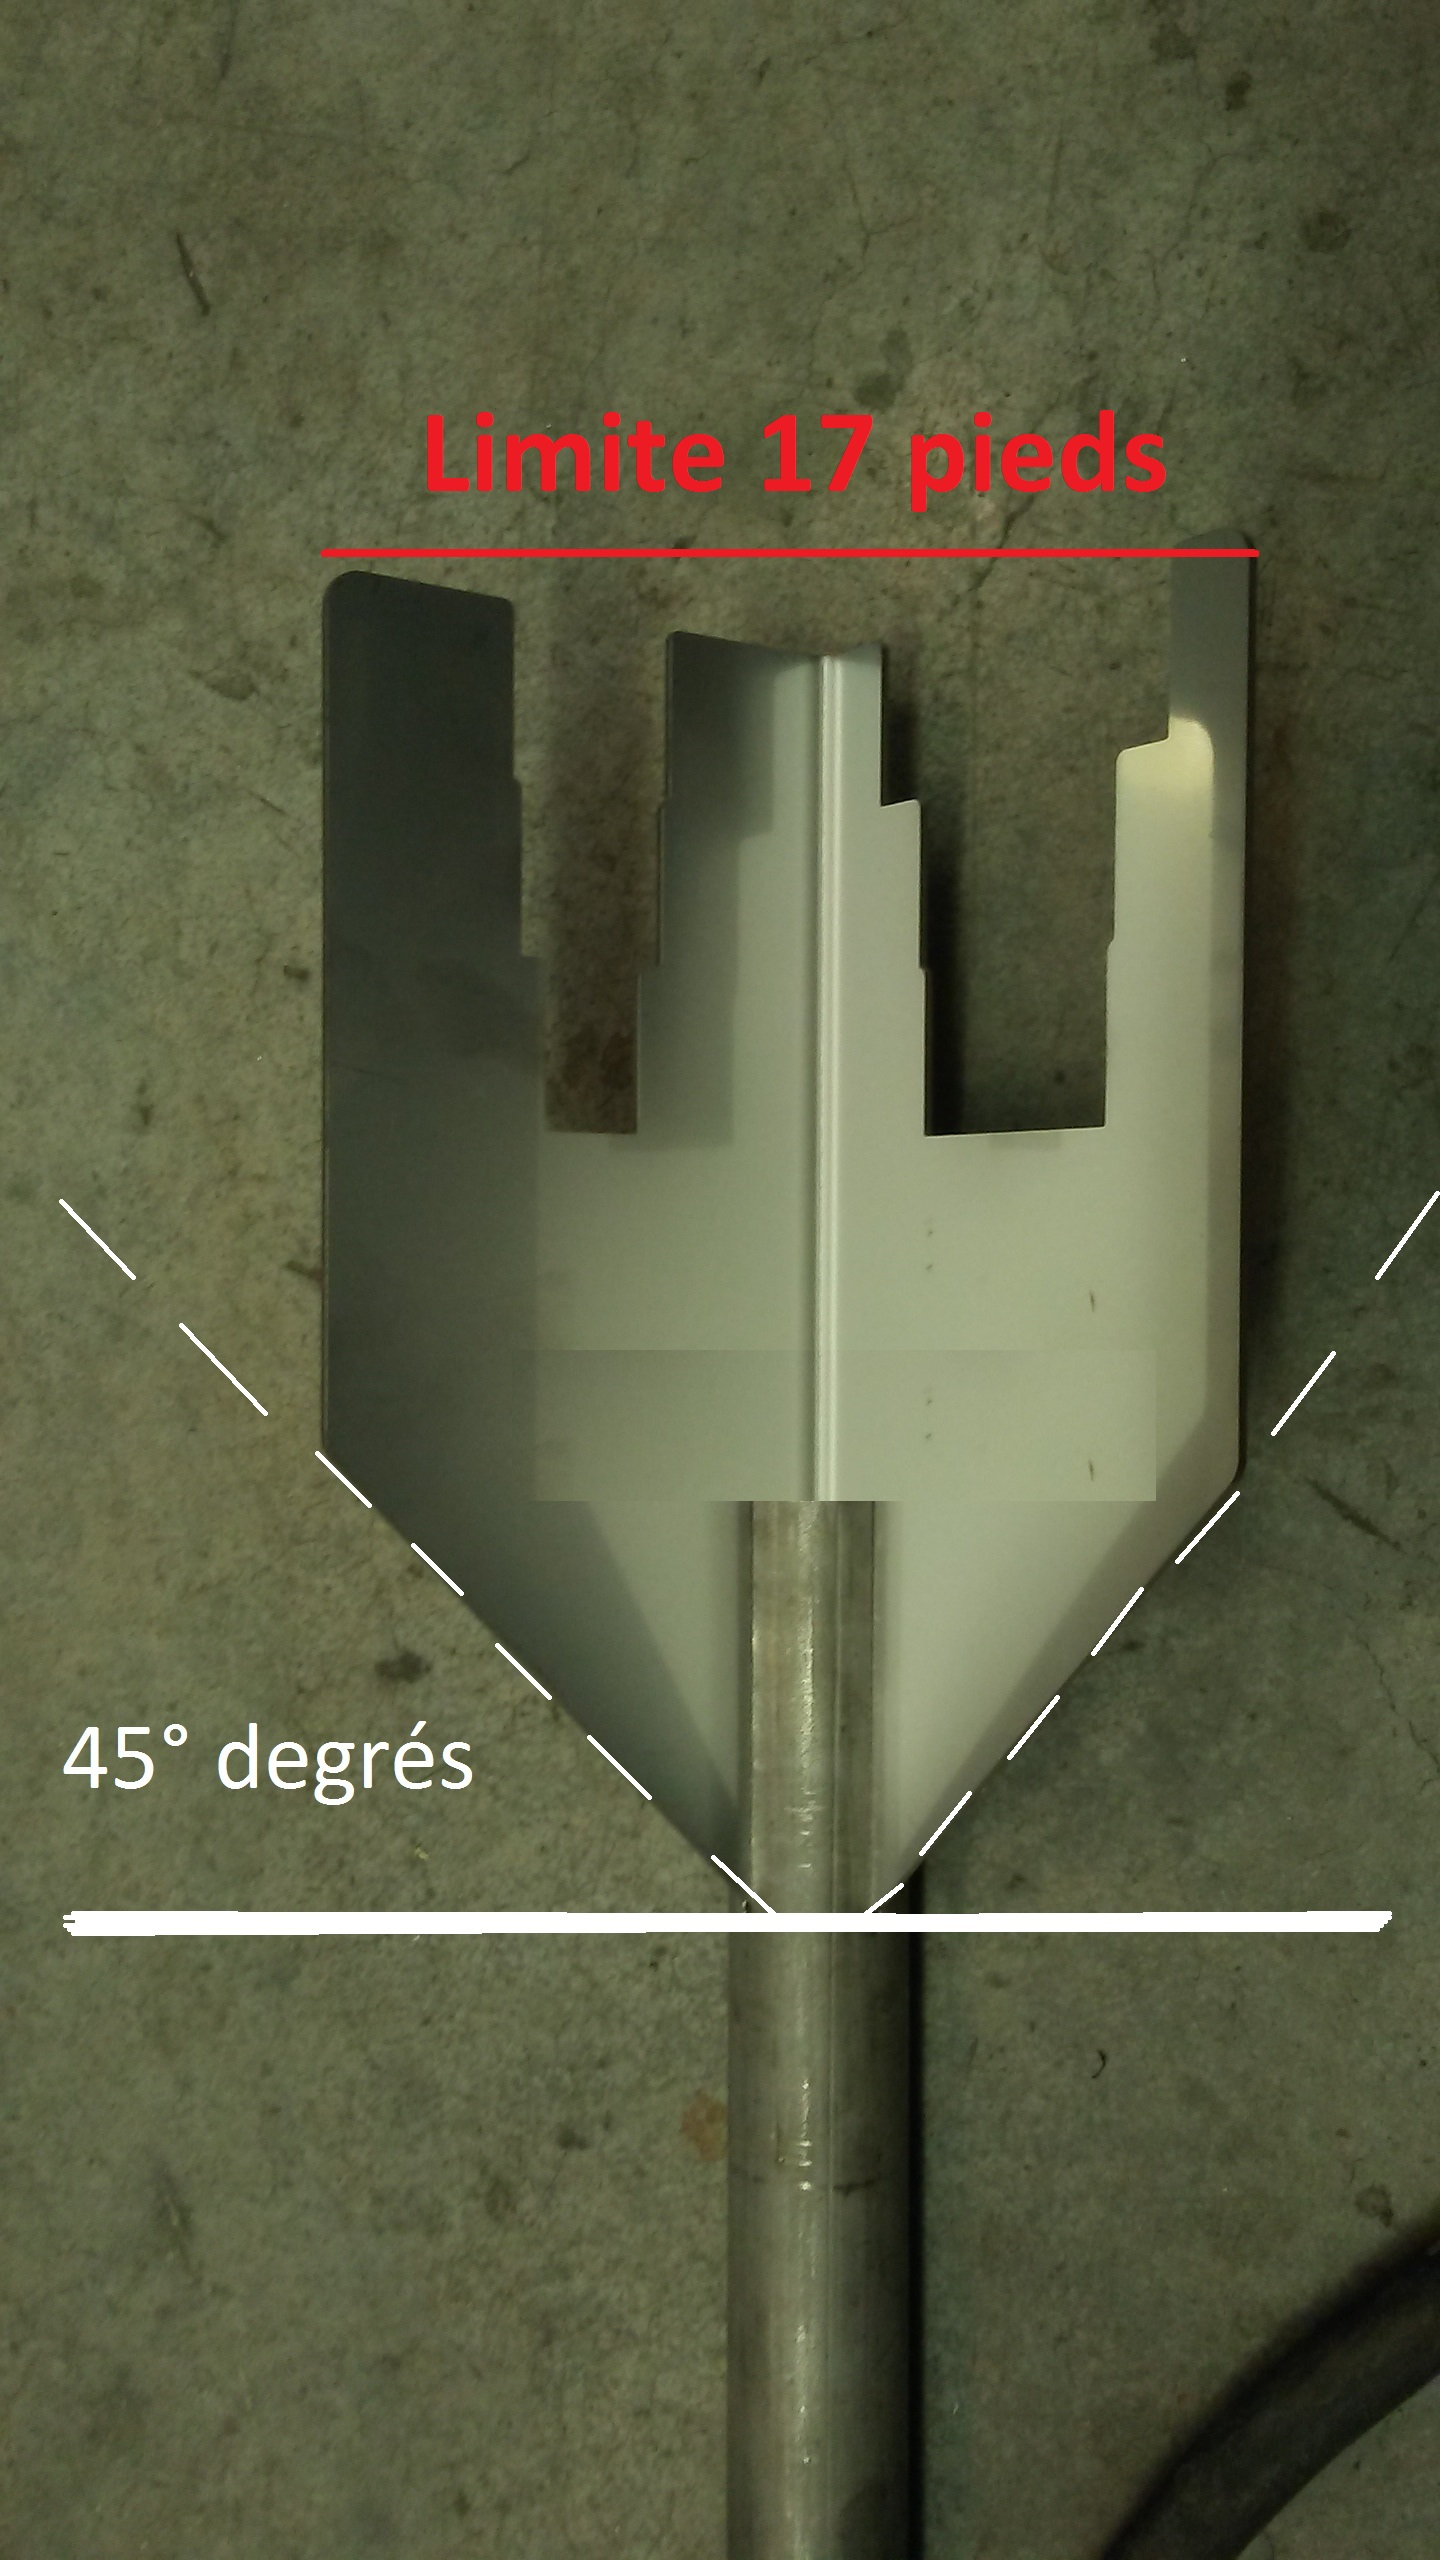
\includegraphics[width=5cm]{Figure4}
	\caption{Gabarit métallique}
	\label{gabarit}
\end{figure}

\subsubsection{Analyse statistique}

Plusieurs données seront récoltées sur les arbres dans toutes les placettes permanentes. Pour l'analyse de ces données, les variables dépendantes seront les suivantes: le numéro d'encoche (grosseur de la branche), l'inclinaison de la branche, et l'état de la branche. Quant aux variables explicatives, il y aura : l'essence, la densité de plantation (plant/ha), l'IQS, l'exposition et la lattitude. Concernant les paramètres environnementaux, nous utiliserons principalement l'exposition, car elle peut favoriser la croissance du houppier sur la face la plus ensoleillée. Étant donné que toute les placettes sont géoréférencées, il sera également possible d'utiliser la lattitude comme variable, dans le but de vérifier le gradient Nord-Sud a une incidence sur la grosseur des noeuds. Par une technique de régression multinomiale, il sera possible d'estimer la proportion des faces se ayant une taille de nœuds donnée pour différents scénarios d'espacements. Il sera ensuite possible d'estimer dans quelle mesure un espacement initial plus large est susceptible d'engendrer des déclassements de la qualité des planches.

\subsection{Modélisation du défilement et de la composition du panier de produits}

À l’aide d’un simulateur d’éclaircies créé par la Direction de la Recherche Forestière, "Simuléclaircies version GS Taktik", il sera possible de déterminer le DHP quadratique moyen et la hauteur dominante des tiges à maturité en fonction: de l’essence, de l’IQS, de la densité de reboisement et du scénario sylvicole (0, 1 ou 2 éclaircies). 

\vspace{12pt}

Afin de simuler la transformation primaire, FPInnovations a développé Optitek, un logiciel qui utilise les données acquises à partir de scanners laser pour donner une représentation tridimensionnelle de la forme réelle de la tige \cite{FPInnovations2014}. Toutefois, ce logiciel demande une compréhension fine de la transformation primaire du bois pour être bien utilisé. Ce niveau de compréhension dépassant le cadre de cette étude, nous utiliserons plutôt une simplification du modèle qui tient compte du DHP et de la hauteur des arbres pour prédire la composition du panier de produits déterminée par Optitek. Ce méta-modèle statistique nommé STATSAW \cite{Auty2014} est paramétré pour l'épinette noire. À défaut d'avoir d'autres modèles, nous utiliserons STATSAW aussi pour l'épinette blanche et le pin gris.

\section{Résultats escomptés}

On s’attend à une relation entre la densité de plantation et les propriétés du bois (proportion de sciage, grosseur des branches). On suppose qu'un espacement initial plus large pourrait donner de meilleurs résultats en terme de rendement en valeur des produits, mais que cela peut dépendre des espèces. Par exemple, puisque le pin gris fait de plus gros noeuds, il est possible que l'\textit{optimum} de densité de plantation se situe à une valeur plus faible d'espacement que 2 mètres. Ces suppositions sont aussi à vérifier pour l'épinette noire et l'épinette blanche. 

\vspace{12pt}

Pour le diamètre de la plus grosse branche, on s'attend à observer une augmentation de la grosseur des branches à de plus fortes densités. En effet, la hausse de la mortalité interspécifique devrait libérer de l'espace aux arbres résiduels et favoriser leurs développement de houppier et donc des branches.

\vspace{12pt}

Le défilement est bien documenté sur les trois essences, ce qui permettra de bien alimenter le simulateur Optitek en données pour prévoir une valeur par arbre. Les ajustements avec le modèle STATSAW étant initialement paramétrés pour l'épinette noire, il y aura nécessairement une incertitude pour l'épinette blanche et le pin gris quant à la projection du panier de produits. Toutefois, on suppose une augmentation de la proportion de sciage pour toutes les essences au fur et à mesure que la densité diminue. 

\section{Conclusion}

À la lumière des résultats obtenus, des recommandations pourront être formulées auprès des praticiens en régions pour les sensibiliser aux effets de la densité de reboisement sur les caractéristiques du bois. En  termes  économiques,  si  les caractéristiques du bois ne se dégradent pas trop rapidement au fur et à mesure qu'on diminue la densité de plantation,  il peut être envisageable d'abaisser le nombre de tiges à l'hectare et donc de réduire les  coûts  de  plantation. Une autre retombée espérée est de pouvoir créer, à long terme, des bois issus de plantations ayant le meilleur panier de produits possible. 

\end{onehalfspace}

\section{Échéancier}

\begin{figure}[H]
	\centering
	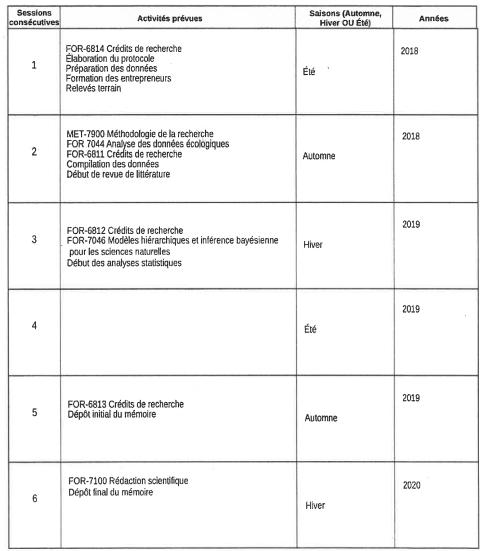
\includegraphics[width=15cm]{Calendrier}
	\caption{Calendrier des activités}
\end{figure}

\newpage

\nocite{*}
\bibliographystyle{unsrt}
\bibliography{biblio}

\end{document}